% Options for packages loaded elsewhere
\PassOptionsToPackage{unicode}{hyperref}
\PassOptionsToPackage{hyphens}{url}
\PassOptionsToPackage{dvipsnames,svgnames,x11names}{xcolor}
%
\documentclass[
  letterpaper,
  DIV=11,
  numbers=noendperiod]{scrartcl}

\usepackage{amsmath,amssymb}
\usepackage{iftex}
\ifPDFTeX
  \usepackage[T1]{fontenc}
  \usepackage[utf8]{inputenc}
  \usepackage{textcomp} % provide euro and other symbols
\else % if luatex or xetex
  \usepackage{unicode-math}
  \defaultfontfeatures{Scale=MatchLowercase}
  \defaultfontfeatures[\rmfamily]{Ligatures=TeX,Scale=1}
\fi
\usepackage{lmodern}
\ifPDFTeX\else  
    % xetex/luatex font selection
\fi
% Use upquote if available, for straight quotes in verbatim environments
\IfFileExists{upquote.sty}{\usepackage{upquote}}{}
\IfFileExists{microtype.sty}{% use microtype if available
  \usepackage[]{microtype}
  \UseMicrotypeSet[protrusion]{basicmath} % disable protrusion for tt fonts
}{}
\makeatletter
\@ifundefined{KOMAClassName}{% if non-KOMA class
  \IfFileExists{parskip.sty}{%
    \usepackage{parskip}
  }{% else
    \setlength{\parindent}{0pt}
    \setlength{\parskip}{6pt plus 2pt minus 1pt}}
}{% if KOMA class
  \KOMAoptions{parskip=half}}
\makeatother
\usepackage{xcolor}
\setlength{\emergencystretch}{3em} % prevent overfull lines
\setcounter{secnumdepth}{-\maxdimen} % remove section numbering
% Make \paragraph and \subparagraph free-standing
\makeatletter
\ifx\paragraph\undefined\else
  \let\oldparagraph\paragraph
  \renewcommand{\paragraph}{
    \@ifstar
      \xxxParagraphStar
      \xxxParagraphNoStar
  }
  \newcommand{\xxxParagraphStar}[1]{\oldparagraph*{#1}\mbox{}}
  \newcommand{\xxxParagraphNoStar}[1]{\oldparagraph{#1}\mbox{}}
\fi
\ifx\subparagraph\undefined\else
  \let\oldsubparagraph\subparagraph
  \renewcommand{\subparagraph}{
    \@ifstar
      \xxxSubParagraphStar
      \xxxSubParagraphNoStar
  }
  \newcommand{\xxxSubParagraphStar}[1]{\oldsubparagraph*{#1}\mbox{}}
  \newcommand{\xxxSubParagraphNoStar}[1]{\oldsubparagraph{#1}\mbox{}}
\fi
\makeatother


\providecommand{\tightlist}{%
  \setlength{\itemsep}{0pt}\setlength{\parskip}{0pt}}\usepackage{longtable,booktabs,array}
\usepackage{calc} % for calculating minipage widths
% Correct order of tables after \paragraph or \subparagraph
\usepackage{etoolbox}
\makeatletter
\patchcmd\longtable{\par}{\if@noskipsec\mbox{}\fi\par}{}{}
\makeatother
% Allow footnotes in longtable head/foot
\IfFileExists{footnotehyper.sty}{\usepackage{footnotehyper}}{\usepackage{footnote}}
\makesavenoteenv{longtable}
\usepackage{graphicx}
\makeatletter
\newsavebox\pandoc@box
\newcommand*\pandocbounded[1]{% scales image to fit in text height/width
  \sbox\pandoc@box{#1}%
  \Gscale@div\@tempa{\textheight}{\dimexpr\ht\pandoc@box+\dp\pandoc@box\relax}%
  \Gscale@div\@tempb{\linewidth}{\wd\pandoc@box}%
  \ifdim\@tempb\p@<\@tempa\p@\let\@tempa\@tempb\fi% select the smaller of both
  \ifdim\@tempa\p@<\p@\scalebox{\@tempa}{\usebox\pandoc@box}%
  \else\usebox{\pandoc@box}%
  \fi%
}
% Set default figure placement to htbp
\def\fps@figure{htbp}
\makeatother

\KOMAoption{captions}{tableheading}
\makeatletter
\@ifpackageloaded{caption}{}{\usepackage{caption}}
\AtBeginDocument{%
\ifdefined\contentsname
  \renewcommand*\contentsname{Table of contents}
\else
  \newcommand\contentsname{Table of contents}
\fi
\ifdefined\listfigurename
  \renewcommand*\listfigurename{List of Figures}
\else
  \newcommand\listfigurename{List of Figures}
\fi
\ifdefined\listtablename
  \renewcommand*\listtablename{List of Tables}
\else
  \newcommand\listtablename{List of Tables}
\fi
\ifdefined\figurename
  \renewcommand*\figurename{Figure}
\else
  \newcommand\figurename{Figure}
\fi
\ifdefined\tablename
  \renewcommand*\tablename{Table}
\else
  \newcommand\tablename{Table}
\fi
}
\@ifpackageloaded{float}{}{\usepackage{float}}
\floatstyle{ruled}
\@ifundefined{c@chapter}{\newfloat{codelisting}{h}{lop}}{\newfloat{codelisting}{h}{lop}[chapter]}
\floatname{codelisting}{Listing}
\newcommand*\listoflistings{\listof{codelisting}{List of Listings}}
\makeatother
\makeatletter
\makeatother
\makeatletter
\@ifpackageloaded{caption}{}{\usepackage{caption}}
\@ifpackageloaded{subcaption}{}{\usepackage{subcaption}}
\makeatother

\usepackage{bookmark}

\IfFileExists{xurl.sty}{\usepackage{xurl}}{} % add URL line breaks if available
\urlstyle{same} % disable monospaced font for URLs
\hypersetup{
  pdftitle={Pairs Trading a  Sparse Synthetic Control},
  colorlinks=true,
  linkcolor={blue},
  filecolor={Maroon},
  citecolor={Blue},
  urlcolor={Blue},
  pdfcreator={LaTeX via pandoc}}


\title{Pairs Trading a Sparse Synthetic Control}
\usepackage{etoolbox}
\makeatletter
\providecommand{\subtitle}[1]{% add subtitle to \maketitle
  \apptocmd{\@title}{\par {\large #1 \par}}{}{}
}
\makeatother
\subtitle{Jesus Villota}
\author{}
\date{}

\begin{document}
\maketitle


\section{Introduction}\label{introduction}

\subsection{Pairs Trading}\label{pairs-trading}

{\textbf{\emph{Definition:}}}

\begin{itemize}
\tightlist
\item
  Widely recognized as a cornerstone of \textbf{\emph{statistical
  arbitrage}}
\item
  Exploits \textbf{\emph{temporary divergences}} in the prices of two
  historically correlated or economically linked assets.
\end{itemize}

{\textbf{\emph{Modus Operandi}}}

\begin{itemize}
\tightlist
\item
  \textbf{\emph{Dollar-neutral}} strategy
\item
  Implies simultaneously going:

  \begin{itemize}
  \tightlist
  \item
    {\textbf{LONG} in the relatively \textbf{undervalued} asset}
  \item
    {\textbf{SHORT} in the relatively \textbf{overvalued} one}
  \end{itemize}
\item
  It aims to profit from the eventual \textbf{\emph{convergence of
  prices}} or from \textbf{\emph{mispricing correction}}
\end{itemize}

\subsection{Limitations}\label{limitations}

{\textbf{\emph{Pairs identification}}}

\begin{itemize}
\tightlist
\item
  \textbf{\emph{Difficult to identify}} pairs of economically linked
  assets
\item
  \textbf{\emph{High-dimensional asset pools}} exacerbate the problem
\end{itemize}

{\textbf{\emph{Time-varying correlations}}}

\begin{itemize}
\tightlist
\item
  Even when a pair is identified, their \textbf{\emph{relationship will
  change over time}}
\end{itemize}

{\textbf{\emph{Sensitivity to noise}}}

\begin{itemize}
\tightlist
\item
  Identifying mispricing in a pair is \textbf{\emph{too sensitive to
  noise}}
\item
  Difficult to separate noise from mispricing
\end{itemize}

{\textbf{\emph{Non-linear dependencies}}}

\begin{itemize}
\tightlist
\item
  Traditional approaches rely on \textbf{\emph{distance}} measures or
  \textbf{\emph{cointegration}}-based criteria
\end{itemize}

\subsection{Research Gap}\label{research-gap}

{\textbf{\emph{Need for strategies that\ldots{}}}}

\begin{itemize}
\tightlist
\item
  Systematically identify latent economic linkages
\item
  Mitigate overfitting in high-dimensional asset pools
\item
  Robust to changing market conditions
\item
  Successfully separate mispricing from noise
\item
  Capture non-linear and tail dependencies
\end{itemize}

\subsection{Research Question}\label{research-question}

Can the integration of \textbf{\emph{sparse synthetic control}} with
\textbf{\emph{copula-based dependence modeling}} improve the performance
of pairs trading strategies?

\subsection{Our Approach}\label{our-approach}

\begin{itemize}
\tightlist
\item
  Novel framework integrating:

  \begin{itemize}
  \tightlist
  \item
    \textsc{\textbf{Sparse synthetic control methods}}
  \item
    \textsc{\textbf{Copula-based dependence modeling}}
  \end{itemize}
\end{itemize}

\begin{itemize}
\tightlist
\item
  Designed to enhance:

  \begin{itemize}
  \tightlist
  \item
    \textbf{\emph{Identification}} of pairs
  \item
    Strategy \textbf{\emph{adaptability}}
  \item
    \textbf{\emph{Risk management}} capabilities
  \item
    Performance \textbf{\emph{stability}}
  \end{itemize}
\end{itemize}

\subsection{Key Methodological
Components}\label{key-methodological-components}

\begin{itemize}
\tightlist
\item
  \textbf{Sparse Synthetic Control}

  \begin{itemize}
  \tightlist
  \item
    Avoids reliance on a fixed or pre-specified partner asset
  \item
    Constructs a \emph{synthetic pair} as a sparse linear combination
    from a donor pool
  \end{itemize}
\end{itemize}

\begin{itemize}
\tightlist
\item
  \textbf{Copula-Based Dependence Framework}

  \begin{itemize}
  \tightlist
  \item
    Captures non-linear relationships between the target \& synthetic
    assets
  \item
    Allows us to compute mispricing probabilities
  \end{itemize}
\end{itemize}

\begin{itemize}
\tightlist
\item
  \textbf{Trading Signal Generation}

  \begin{itemize}
  \tightlist
  \item
    Based on relative mispricing between target and synthetic assets
  \item
    Designed to filter market noise
  \end{itemize}
\end{itemize}

\section{Literature Review}\label{literature-review}

\subsection{Literature Review}\label{literature-review-1}

{\textbf{Classical Pairs Trading}}

\begin{itemize}
\tightlist
\item
  \textbf{Gatev et al.~(1998)}:

  \begin{itemize}
  \tightlist
  \item
    \emph{First comprehensive academic study}
  \item
    \emph{Documented 11\% annual excess returns (1962-2002)}
  \item
    \emph{Established distance-based methodology}
  \end{itemize}
\end{itemize}

\begin{itemize}
\tightlist
\item
  \textbf{Elliott et al.~(2005)}:

  \begin{itemize}
  \tightlist
  \item
    \emph{introduced a mean-reverting Gaussian Markov chain model for
    spread dynamics}
  \item
    \emph{established analytical methods for parameter estimation using
    EM}
  \end{itemize}
\end{itemize}

{\textbf{Empirical Validations}}

\begin{itemize}
\tightlist
\item
  \textbf{Chen et al.~(2019)} \emph{reports large abnormal returns
  driven by short-term reversals and pairs momentum effects}
\end{itemize}

\begin{itemize}
\tightlist
\item
  \textbf{Do et al.~(2010)}: \emph{showed that pairs trading remains
  viable in turbulent periods}
\end{itemize}

\begin{itemize}
\tightlist
\item
  \textbf{Krauss (2016) \& Rad et al.~(2016)}: \emph{confirmed that
  distance, cointegration, and copula-based strategies can yield
  significant alpha but exhibit important differences regarding
  convergence speed and trading frequencies.}
\end{itemize}

\subsection{Literature Review}\label{literature-review-2}

{\textbf{Cointegration Approach}}

\begin{itemize}
\tightlist
\item
  \textbf{Vidyamurthy (2004)}: \emph{seminal application to equity
  markets}
\item
  \textbf{Caldeira and Moura (2013)}: \emph{Brazilian market
  application}
\item
  \textbf{Huck and Afawubo (2014)}: \emph{cointegration outperforms
  distance methods}
\item
  \textbf{Cartea and Jaimungal (2015)}: \emph{Optimal dynamic investment
  strategies}
\item
  \textbf{Lintilhac (2016)}: \emph{Cryptocurrency applications}
\end{itemize}

{\textbf{Copula-Based Methods}}

\begin{itemize}
\tightlist
\item
  \textbf{Min and Czado (2010)}: \emph{Bayesian inference for
  pair-copulas}
\item
  \textbf{Stander et al.~(2013)}: \emph{Mispricing detection framework}
\item
  \textbf{Liew and Wu (2013) \& Xie et al.~(2016)}: \emph{Superior tail
  dependencies}
\item
  \textbf{Krauss and Stubinger (2017) \& Zhi et al.~(2017)}:
  \emph{Adaptive thresholds}
\item
  \textbf{Recent extensions}:

  \begin{itemize}
  \tightlist
  \item
    Mixed copulas (da Silva et al., 2023)
  \item
    ARMA-GARCH integration (Wang and Ding, 2023)
  \item
    Cryptocurrency applications (Tadi and Witzany, 2025)
  \end{itemize}
\end{itemize}

\subsection{Literature Review}\label{literature-review-3}

{\textbf{Advanced Modeling Techniques}}

\begin{itemize}
\tightlist
\item
  \textbf{Do (2006)}: \emph{Stochastic residual spread models}
\item
  \textbf{Zeng and Lee (2014)}: \emph{Optimal threshold determination}
\item
  \textbf{Johansson et al.~(2024)}: \emph{Convex-concave optimization
  for multi-asset statistical arbitrage}
\item
  \textbf{Machine Learning Integration}:

  \begin{itemize}
  \tightlist
  \item
    \emph{OPTICS clustering to constrain search space} (Sarmento and
    Horta, 2020)
  \item
    \emph{Reinforcement Learning for automated pairs selection} (Han et
    al., 2023)
  \item
    \emph{Graphical matching to reduce overlap among pairs} (Qureshi and
    Zaman, 2024)
  \end{itemize}
\end{itemize}

{\textbf{Replication Methods}}

\begin{itemize}
\tightlist
\item
  \textbf{Alexander (1999), Alexander and Dimitriu (2002)}:
  \emph{classical treatment connecting cointegration analysis and
  hedging tasks}
\item
  \textbf{Alexander and Dimitriu (2005a, 2005b)}: \emph{investigate how
  cointegration outperforms traditional techniques in crafting robust
  index trackers and exploiting time-varying market regimes}
\item
  \textbf{Shu et al.~(2020)}: \emph{shows that sparse solutions across a
  large universe can reduce transaction costs}
\item
  \textbf{Bradrania et al.~(2021)}: \emph{dynamic selection methods for
  index constituents using machine learning}
\end{itemize}

\subsection{Research Positioning}\label{research-positioning}

\emph{Our contribution\ldots{}}

\begin{itemize}
\tightlist
\item
  Integrates sparse synthetic control with copula-based dependence
  modeling
\item
  Overcomes the cumbersome pairs identification process
\item
  Enhances adaptability to structural breaks and complex dependencies
\item
  Provides systematic framework for high-dimensional asset pools
\end{itemize}

\section{Methodology}\label{methodology}

\subsection{Sparse Synthetic Control}\label{sparse-synthetic-control}

\begin{itemize}
\tightlist
\item
  Let \(\mathbf{y} = [y_t]_{t=1}^T\) be the log-price of target asset
\item
  Let \(\mathbf{X} = [x_{1t}, ..., x_{Nt}]_{t=1}^T\) be the log-prices
  of donor assets
\item
  Build synthetic asset \(\mathbf{y}^*\) as:
\end{itemize}

\[
y_t^* = \sum_{i=1}^N w_i^* x_{it} \quad \text{for } t=1,...,T
\]

\begin{itemize}
\tightlist
\item
  weights \(\mathbf{w}^*=[w_1^*, ..., w_N^*]'\) solve:
\end{itemize}

\[
\mathbf{w}^* = \arg\min_{\mathbf{w} \in \mathbb{R}^N} \left\{\sum_{t=1}^T \left(y_t - \sum_{i=1}^N w_i x_{it}\right)^2 + \lambda\|\mathbf{w}\|_1\right\} 
\quad \text{s.t.} \quad \mathbf{1}^\top \mathbf{w} = 1
\]

\subsection{Key Features}\label{key-features}

\begin{itemize}
\tightlist
\item
  \textbf{\(\ell_1\) Regularization (LASSO)}

  \begin{itemize}
  \tightlist
  \item
    Induces sparsity through non-differentiability at origin
  \item
    Automatically selects most relevant assets
  \end{itemize}
\item
  \textbf{Optimization Properties}

  \begin{itemize}
  \tightlist
  \item
    Unique solution (convex problem)
  \item
    Direct sparsity control via \(\lambda\)
  \item
    Portfolio interpretation (\(\mathbf{1}^\top \mathbf{w} = 1\))
  \end{itemize}
\item
  \textbf{Implementation}

  \begin{itemize}
  \tightlist
  \item
    Support identification via thresholding: \[
    \mathcal{I} = \{i \in \{1,...,N\} : |w^*_i| > \epsilon\}
    \]
  \item
    Efficient solution via proximal algorithms
  \end{itemize}
\end{itemize}

\subsection{Empirical Application}\label{empirical-application}

\begin{itemize}
\tightlist
\item
  \textbf{Data}: S\&P500 daily adjusted-close prices
\item
  \textbf{Target}: NVIDIA (NVDA)
\item
  \textbf{Period}: Jan 2010 - Jan 2025
\item
  \textbf{Split}: 70\% training, 30\% testing
\item
  \textbf{Result}: 27 stocks selected
\end{itemize}

\subsection{Synthetic Control Model
Weights}\label{synthetic-control-model-weights}

Ticker

Company

Weight (\%)

AME

Ametek

41.08

LUV

Southwest Airlines

33.31

TFC

Truist Financial

25.60

AEP

American Electric Power

21.69

ADM

Archer Daniels Midland

20.56

RSG

Republic Services

18.42

AXP

American Express

18.10

LLY

Lilly (Eli)

14.74

C

Citigroup

9.67

VRSN

Verisign

7.77

MTB

M\&T Bank

7.38

FE

FirstEnergy

7.16

FIS

Fidelity National Info

5.21

PARA

Paramount Global

4.48

Ticker

Company

Weight (\%)

TXT

Textron

2.21

STX

Seagate Technology

0.26

BIIB

Biogen

0.16

NFLX

Netflix

-1.04

FDX

FedEx

-2.39

UDR

UDR, Inc.

-3.95

V

Visa Inc.

-5.43

CNP

CenterPoint Energy

-7.75

MS

Morgan Stanley

-16.21

NI

NiSource

-16.35

WMT

Walmart

-16.65

UNP

Union Pacific

-25.77

ADSK

Autodesk

-42.25

Total

100.00

\subsection{Target vs Synthetic
Log-Prices}\label{target-vs-synthetic-log-prices}

\begin{center}
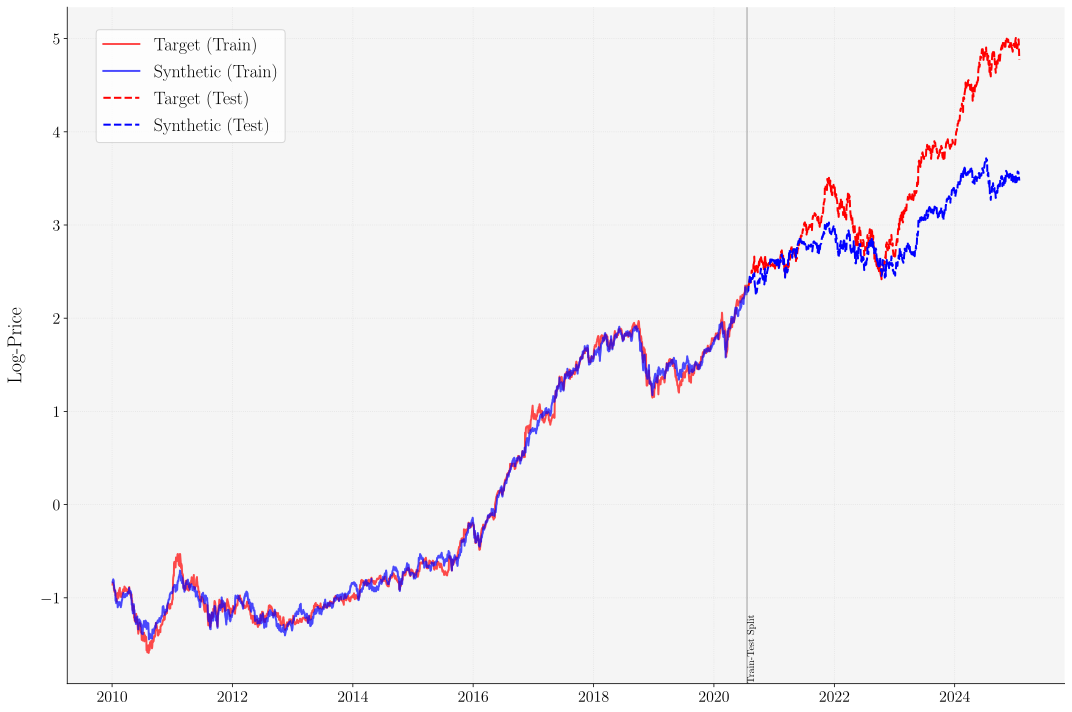
\includegraphics[width=1\linewidth,height=\textheight,keepaspectratio]{simple_Presentation_files/mediabag/images/converted/target_synthetic_prices_NVDA.pdf}
\end{center}

\subsection{Copula-based Modeling}\label{copula-based-modeling}

\begin{itemize}
\tightlist
\item
  Traditional pairs-trading approaches rely on \emph{linear correlation}
  and \emph{cointegration measures}

  \begin{itemize}
  \tightlist
  \item
    {\textbf{Limitations}}

    \begin{itemize}
    \tightlist
    \item
      Restrictive assumptions about joint distributions
    \item
      Poor performance during market stress
    \item
      Miss asymmetric tail dependencies
    \end{itemize}
  \end{itemize}

  \begin{itemize}
  \tightlist
  \item
    {\textbf{Solution: Copula-based dependence modeling}}

    \begin{itemize}
    \tightlist
    \item
      Decouples marginal distributions from joint dependence
    \item
      Captures non-linear interactions
    \item
      Allows to quantify mispricing probabilities
    \end{itemize}
  \end{itemize}
\end{itemize}

\subsection{Sklar's Theorem}\label{sklars-theorem}

\begin{itemize}
\tightlist
\item
  Let \((\Omega, \mathcal{F}, \mathbb{P})\) be a probability space.
\end{itemize}

\begin{itemize}
\tightlist
\item
  Let \(R, R^*: \Omega \to \mathbb{R}\) be RVs representing
  \textbf{\emph{target}} and \textbf{\emph{synthetic}} log-returns.
\end{itemize}

\begin{itemize}
\tightlist
\item
  Let \(F_R\) and \(F_{R^*}\) denote their respective cumulative
  distribution functions (CDFs).
\end{itemize}

\begin{itemize}
\item
  Then, for the joint CDF \(F_{R,R^*}\), there exists a copula
  \(C: [0,1]^2 \to [0,1]\) s.t.:
  \[F_{R,R^*}(r,r^*) = C(F_R(r), F_{R^*}(r^*)) \quad \forall r,r^* \in \mathbb{R}\]
\item
  If \(F_R\) and \(F_{R^*}\) are continuous, then \(C\) is unique.
\end{itemize}

\begin{itemize}
\tightlist
\item
  Conversely, if \(C\) is a copula and \(F_R\), \(F_{R^*}\) are CDFs,
  then \(F_{R,R^*}\) defined above is a joint CDF with margins \(F_R\)
  and \(F_{R^*}\).
\end{itemize}

\subsection{}\label{section}

\begin{itemize}
\tightlist
\item
  When uniqueness holds, by the \textbf{\emph{Probability Integral
  Transform}}:
\end{itemize}

\[
C(u,v) = \mathbb P( F_R(R) \leq u, F_{R^*}(R^*) \leq v) 
\quad \text{for} \quad
(u,v)\in[0,1]^2
.
\]

\begin{itemize}
\tightlist
\item
  When it exists, the \textbf{\emph{copula density}}
  \(c:[0,1]^2\to\mathbb R_+\) is given by
\end{itemize}

\[
   c(u,v) = \frac{\partial^2 C(u,v)}{\partial u \partial v},
\]

\begin{itemize}
\tightlist
\item
  Then, the \textbf{\emph{joint density}} can be decomposed as:
\end{itemize}

\[
f_{R,R^*}(r,r^*) = c(F_R(r), F_{R^*}(r^*)) f_R(r)f_{R^*}(r^*)
\]

\subsection{Marginal Distribution
Estimation}\label{marginal-distribution-estimation}

\begin{enumerate}
\def\labelenumi{\arabic{enumi}.}
\item
  \textbf{Compute log-returns}: \[
  r_t = y_t - y_{t-1} \quad \text{and} \quad r_t^* = y_t^* - y_{t-1}^* 
  % \quad \quad t=2,...,T
  \]
\item
  \textbf{Estimate ECDFs}: \begin{align}
  \hat{F}_{R}(r) &= \frac{1}{T-1} \sum_{t=2}^T \mathbb{I}(r_t \leq r)
  \\
  \hat{F}_{R^*}(r^*) &= \frac{1}{T-1} \sum_{t=2}^T \mathbb{I}(r_t^* \leq r^*)
  \end{align}
\item
  \textbf{Transform to uniforms}: \[
  u_t = \hat{F}_R(r_t) \quad \text{and} \quad v_t = \hat{F}_{R^*}(r_t^*)
  \]
\end{enumerate}

\subsection{CDF Scatterplot: Returns Vs.
Prices}\label{cdf-scatterplot-returns-vs.-prices}

\begin{center}
\includegraphics[width=1\linewidth,height=\textheight,keepaspectratio]{simple_Presentation_files/mediabag/images/converted/CDF_scatter_comparison.pdf}
\end{center}

\subsection{Empirical CDFs: Returns Vs.
Prices}\label{empirical-cdfs-returns-vs.-prices}

\begin{center}
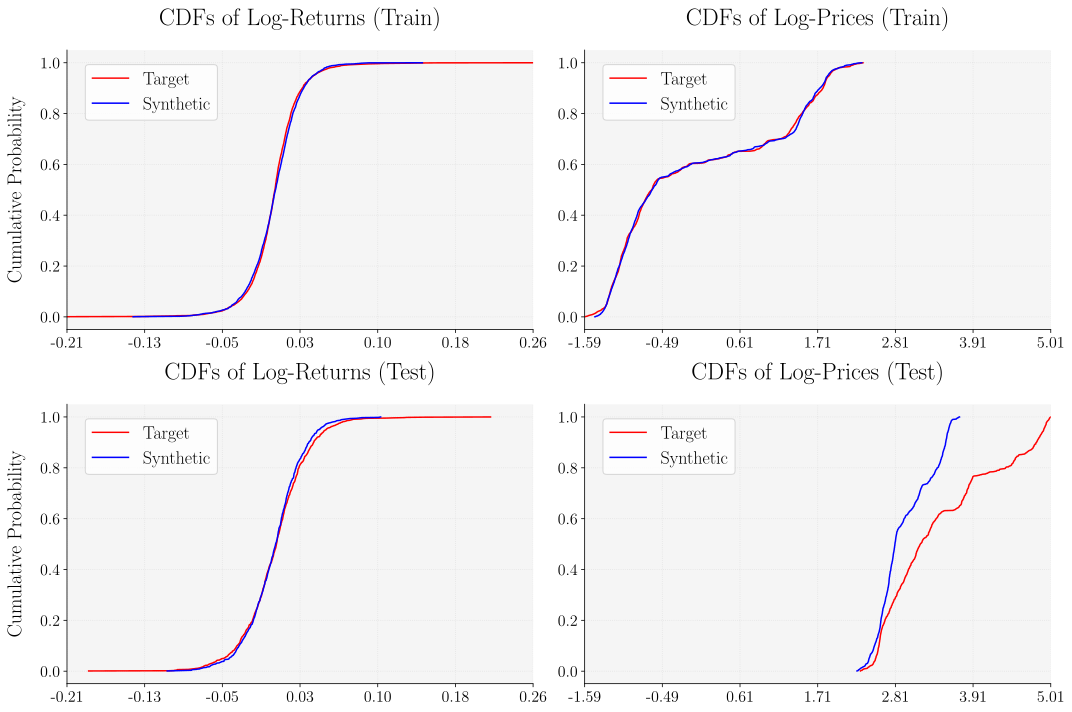
\includegraphics[width=0.5\linewidth,height=\textheight,keepaspectratio]{simple_Presentation_files/mediabag/images/converted/all_CDFs_comparison.pdf}
\end{center}

\subsection{Maximum Likelihood
Estimation}\label{maximum-likelihood-estimation}

For each copula family
\(\mathcal{C} = \{C_\theta : \theta \in \Theta\}\), estimate parameters
via:

\[\hat{\theta} = \arg\max_{\theta \in \Theta} \ell(\theta | \mathbf{u,v})\]

where the log-likelihood is:

\[\ell(\theta| \mathbf{u,v}) := \sum_{t=2}^T \ln c_\theta(u_t, v_t)\]

and \(c_\theta(u,v)\) is the copula density:

\[c_\theta(u,v) = \frac{\partial^2 C_\theta}{\partial u \partial v}(u,v)\]

\subsection{Elliptical Copulas}\label{elliptical-copulas}

\textbf{Gaussian Copula}: \(\Theta = \{\rho \in (-1,1)\}\)
\[c_\rho^{Gauss}(u,v) = \frac{1}{\sqrt{1-\rho^2}} \exp\left(-\frac{\zeta_u^2 + \zeta_v^2 - 2\rho\zeta_u\zeta_v}{2(1-\rho^2)} + \frac{\zeta_u^2 + \zeta_v^2}{2}\right)\]
where \(\zeta_u = \Phi^{-1}(u)\), \(\zeta_v = \Phi^{-1}(v)\)

\textbf{Student-t Copula}: \(\Theta = \{\rho \in (-1,1), \nu > 2\}\)
\[c_{\rho,\nu}^{t}(u,v) = \frac{\Gamma(\frac{\nu+2}{2})\Gamma(\frac{\nu}{2})}{\sqrt{1-\rho^2}\Gamma(\frac{\nu+1}{2})^2} 
\frac{(1 + \frac{\zeta_u^2 + \zeta_v^2 - 2\rho\zeta_u\zeta_v}{\nu(1-\rho^2)})^{-(\nu+2)/2}}{\prod_{i\in\{u,v\}} (1 + \frac{\zeta_i^2}{\nu})^{-(\nu+1)/2}}
\] where \(\zeta_u = t_\nu^{-1}(u)\), \(\zeta_v = t_\nu^{-1}(v)\)

\subsection{Archimedean Copulas}\label{archimedean-copulas}

For generator function \(\psi_\theta\),
\[C_\theta(u,v) = \psi_\theta(\psi_\theta^{-1}(u) + \psi_\theta^{-1}(v))\]

Family

Parameter Range

Generator Function

Clayton

\(\Theta = (0, \infty)\)

\(\psi_\theta(t) = (1 + t)^{-1/\theta}\)

Gumbel

\(\Theta = [1, \infty)\)

\(\psi_\theta(t) = \exp(-t^{1/\theta})\)

Frank

\(\Theta = \mathbb{R}\setminus\{0\}\)

\(\psi_\theta(t) = -\frac{1}{\theta}\ln(1 - (1 - e^{-\theta})e^{-t})\)

Joe

\(\Theta = [1, \infty)\)

\(\psi_\theta(t) = 1 - (1 - e^{-t})^{1/\theta}\)

\subsection{Mixed Copulas}\label{mixed-copulas}

\begin{itemize}
\tightlist
\item
  N14: Rotated Clayton-Gumbel mixture with
  \(\Theta \subset \mathbb{R}^2_+\)
\end{itemize}

\subsection{Characterization of
Copulas}\label{characterization-of-copulas}

\textsc{\textbf{Elliptical Copulas}}

\begin{itemize}
\tightlist
\item
  \textbf{Gaussian Copula}

  \begin{itemize}
  \tightlist
  \item
    Symmetric dependence
  \item
    Light tails
  \end{itemize}
\end{itemize}

\begin{itemize}
\tightlist
\item
  \textbf{Student-t Copula}

  \begin{itemize}
  \tightlist
  \item
    Symmetric dependence
  \item
    Heavy tails
  \end{itemize}
\end{itemize}

\textsc{\textbf{Archimedean Copulas}}

\begin{itemize}
\tightlist
\item
  \textbf{Clayton}

  \begin{itemize}
  \tightlist
  \item
    Asymmetric, lower tail dependence
  \end{itemize}
\item
  \textbf{Gumbel}

  \begin{itemize}
  \tightlist
  \item
    Asymmetric, upper tail dependence
  \end{itemize}
\item
  \textbf{Joe}

  \begin{itemize}
  \tightlist
  \item
    Asymmetric, strong upper tail dependence
  \end{itemize}
\item
  \textbf{Frank}

  \begin{itemize}
  \tightlist
  \item
    Symmetric, no tail dependence
  \end{itemize}
\end{itemize}

\textsc{\textbf{Mixed Copula (N14) }}

\begin{itemize}
\tightlist
\item
  Asymmetric tail dependence
\end{itemize}

\subsection{Calibrated Copula Density
Heatmaps}\label{calibrated-copula-density-heatmaps}

\begin{center}
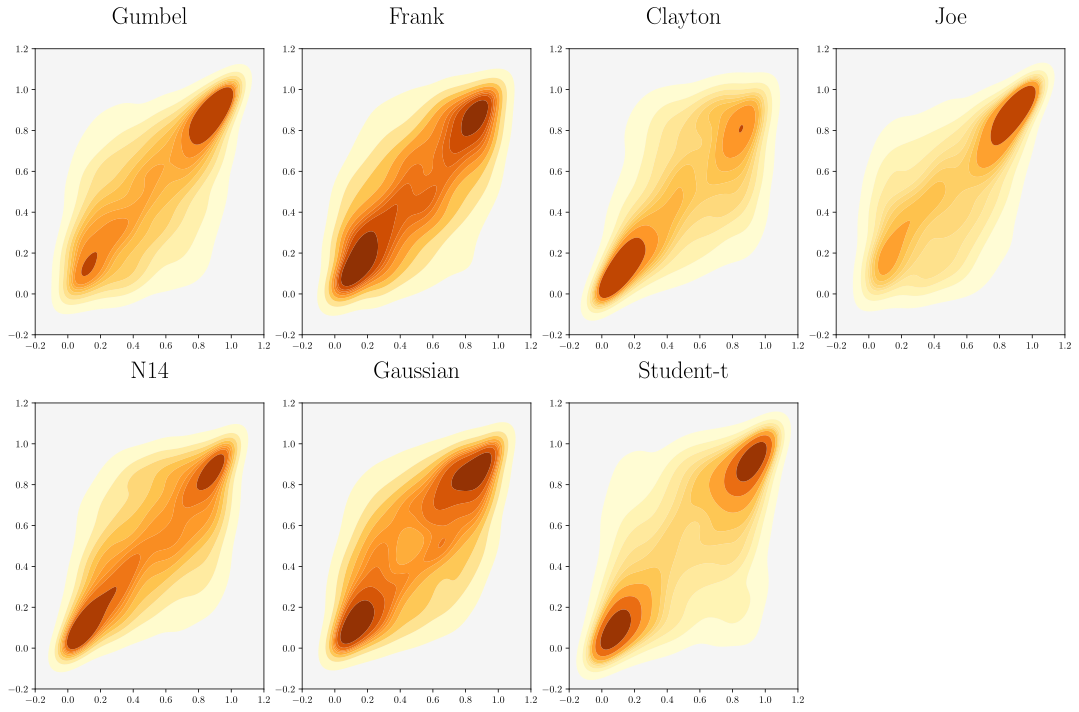
\includegraphics[width=0.5\linewidth,height=\textheight,keepaspectratio]{simple_Presentation_files/mediabag/images/converted/copula_samples_comparison.pdf}
\end{center}

\subsection{Model Selection}\label{model-selection}

\textbf{Information Criteria}:

\[
\begin{array}{ll}
\text{AIC} &= 2k - 2\ell(\hat{\theta}|\mathbf{u,v})
\\
\text{SIC} &= k\ln(T-1) - 2\ell(\hat{\theta}|\mathbf{u,v})
\\
\text{HQIC} &= 2k\ln(\ln T-1) - 2\ell(\hat{\theta}|\mathbf{u,v})
\end{array}
\]

\textbf{Key Findings}:

\begin{itemize}
\tightlist
\item
  Student-t copula provides best fit, followed by N14, Gaussian and
  Frank
\item
  Elliptical copulas provide a better fit than Archimedean copulas
\item
  Heavy tails are significant
\item
  Symmetric dependence structure dominates
\item
  Tail dependence is more relevant than symmetry (N14 \textgreater{}
  Gaussian, Frank)
\end{itemize}

\subsection{Copula Fitting Results}\label{copula-fitting-results}

Copula

SIC

AIC

HQIC

Joe

-671.50

-677.39

-675.26

Clayton

-1168.92

-1174.80

-1172.67

Gumbel

-1210.02

-1215.90

-1213.78

Frank

-1212.68

-1218.56

-1216.43

Gaussian

-1337.69

-1343.57

-1341.44

N14

-1425.18

-1431.06

-1428.94

Student-t

-1427.05

-1432.94

-1430.81

\section{Trading Strategy}\label{trading-strategy}

\subsection{Pairs Trading via Mispricing
Indices}\label{pairs-trading-via-mispricing-indices}

\begin{itemize}
\tightlist
\item
  We adapt the mispricing index (MI) strategy from Xie et al.~(2016) to
  our setting
\end{itemize}

\begin{itemize}
\tightlist
\item
  We trade a target asset (with returns \(R_t\)) against its synthetic
  counterpart (with returns \(R_t^*\)).
\end{itemize}

\begin{itemize}
\tightlist
\item
  While the strategy might initially appear unconventional, it hinges on
  interpreting conditional probabilities of daily returns as an evolving
  measure of relative mispricing.
\end{itemize}

\subsection{Mispricing Index (MI)}\label{mispricing-index-mi}

\begin{itemize}
\item
  Two conditional mispricing indices
\item
  \(MI_t^{R \mid R^*}\Rightarrow\) \emph{How ``mispriced'' is the
  \textbf{target asset} today conditional on today's \textbf{synthetic
  return}?} \[
  MI_t^{R \mid R^*} := \mathbb{P}(R_t \leq r_t \mid R_t^* = r_t^*) = \frac{\partial C_{\hat{\theta}}(F_R(r_t), F_{R^*}(r_t^*))}{\partial F_{R^*}(r_t^*)}
  \]
\end{itemize}

\begin{itemize}
\tightlist
\item
  \(MI_t^{R^* \mid R}\Rightarrow\) \emph{How ``mispriced'' is the
  \textbf{synthetic asset} today conditional on today's \textbf{target
  return}?}
\end{itemize}

\[
MI_t^{R^* \mid R} := \mathbb{P}(R_t^* \leq r_t^* \mid R_t = r_t) = \frac{\partial C_{\hat{\theta}}(F_R(r_t), F_{R^*}(r_t^*))}{\partial F_R(r_t)}
\]

\subsection{Cumulative Mispricing Index
(CMI)}\label{cumulative-mispricing-index-cmi}

\begin{itemize}
\tightlist
\item
  Individual MI reflects only instantaneous view
\item
  Solution:

  \begin{itemize}
  \tightlist
  \item
    Accumulate signals over time to track persistent mispricing
  \item
    Reset them to zero after position is closed to prevent stale signals
  \end{itemize}
\end{itemize}

\begin{itemize}
\tightlist
\item
  This defines a \textbf{Cumulative Mispricing Index} (CMI) for each
  asset:
\end{itemize}

\begin{align}
\mathrm{CMI}^{R}_{t} &=
\begin{cases}
\mathrm{CMI}^{R}_{t-1} + (MI_t^{R\mid R^*} - 0.5), & \text{if no position reset at time } t,\\
0, & \text{if a position is closed at } t,
\end{cases}
\\[1.em]
\mathrm{CMI}^{R^*}_{t} &=
\begin{cases}
\mathrm{CMI}^{R^*}_{t-1} + (MI_t^{R^*\mid R} - 0.5), & \text{if no position reset at time } t,\\
0, & \text{if a position is closed at } t.
\end{cases}
\end{align}

where \(CMI_0^R = CMI_0^{R^*} = 0\).

\subsection{Trading Logic - Signal
Generation}\label{trading-logic---signal-generation}

\begin{itemize}
\tightlist
\item
  \textbf{``Or-Or'' Logic}: Proposed by Xie et al.~(2016)

  \begin{itemize}
  \tightlist
  \item
    Trades are initiated when either asset is shows mispricing
  \item
    Positions are closed when either asset corrects
  \end{itemize}
\end{itemize}

\begin{itemize}
\tightlist
\item
  \textbf{``And-Or'' Logic}: Proposed by Rad et al.~(2016)

  \begin{itemize}
  \tightlist
  \item
    Requires concurrent signals from both assets to open positions
  \item
    Mispricing correction in either asset triggers position closure
  \item
    This logic is more conservative \& yields \emph{more robust
    performance}
  \end{itemize}
\end{itemize}

\begin{itemize}
\tightlist
\item
  \textbf{Parameters}:

  \begin{itemize}
  \tightlist
  \item
    Entry thresholds: \((D_l, D_u) = (-0.6, 0.6)\)
  \item
    Stop-loss boundaries: \((S_l, S_u) = (-2, 2)\)
  \end{itemize}
\end{itemize}

\subsection{Trading Rule}\label{trading-rule}

Trading Rule given the current CMIs (\(\mathrm{CMI}_t^R\),
\(\mathrm{CMI}_t^{R^*}\)) and previous signal (\(TR_{t-1}\)):

\begin{align*}
&TR_t(\text{CMI}_t^R, \text{CMI}_t^{R^*}, TR_{t-1}; D_l, D_u, S_l, S_u) 
=
\\[0.2em]\nonumber
&\begin{cases}
+1 & \text{if} ~  
(\text{CMI}_t^R \leq  D_l 
~\text{and}~ 
\text{CMI}_t^{R^*} \geq D_u)
\\
-1 & \text{if} ~ 
(\text{CMI}_t^R \geq D_u 
~\text{and}~ 
\text{CMI}_t^{R^*} \leq D_l)
\\
0 & \text{if}~
\begin{cases}
\biggl\{
TR_{t-1}=1 
~~~\text{and}~ 
\bigl[
(\underbrace{\text{CMI}_t^R\geq 0 ~\text{or}~ \text{CMI}_t^{R^*}\leq 0}_{\text{take profit}})
~\text{or}~
(\underbrace{\text{CMI}_t^R\leq S_l ~\text{or}~ \text{CMI}_t^{R^*}\geq S_u}_{\text{stop loss}})
\bigr]
\biggr\}
,\text{or}
\\
\biggl\{
TR_{t-1}=-1 
~\text{and}~ 
\bigl[
(\underbrace{\text{CMI}_t^R\leq 0 ~\text{or}~ \text{CMI}_t^{R^*}\geq 0}_{\text{take profit}})
~\text{or}~
(\underbrace{\text{CMI}_t^R\geq S_u ~\text{or}~ \text{CMI}_t^{R^*}\leq S_l}_{\text{stop loss}})
\bigr]
\biggr\}
\end{cases}
\\
TR_{t-1} & \text{otherwise}
\end{cases}
\end{align*}

\subsection{Position Entry and Exit
Conditions}\label{position-entry-and-exit-conditions}

\begin{itemize}
\tightlist
\item
  \textbf{Long target/Short synthetic (+1)}:

  \begin{itemize}
  \tightlist
  \item
    Target \emph{underpriced} (\(\mathrm{CMI}_t^R \leq D_l\))
    \textbf{AND} Synthetic \emph{overpriced}
    (\(\mathrm{CMI}_t^{R^*} \geq D_u\))
  \end{itemize}
\end{itemize}

\begin{itemize}
\tightlist
\item
  \textbf{Short target/Long synthetic (-1)}:

  \begin{itemize}
  \tightlist
  \item
    Target \emph{overpriced} (\(\mathrm{CMI}_t^R \geq D_u\))
    \textbf{AND} Synthetic \emph{underpriced}
    (\(\mathrm{CMI}_t^{R^*} \leq D_l\))
  \end{itemize}
\end{itemize}

\begin{itemize}
\tightlist
\item
  \textbf{Exit position (0)}: Triggered by either:

  \begin{itemize}
  \tightlist
  \item
    \textbf{Take profit}: Either CMI crosses zero (\emph{price
    correction})
  \item
    \textbf{Stop loss}: Either CMI exceeds stop-loss boundaries
  \end{itemize}
\end{itemize}

\subsection{Strategy Implementation}\label{strategy-implementation}

\begin{enumerate}
\def\labelenumi{\arabic{enumi}.}
\tightlist
\item
  \textbf{Daily process}:

  \begin{itemize}
  \tightlist
  \item
    Obtain returns for target (\(r_t\)) and compute synthetic returns
    (\(r_t^*\))
  \item
    Transform to uniform margins: \(u_t = \hat{F}_R(r_t)\),
    \(v_t = \hat{F}_{R^*}(r_t^*)\)
  \item
    Compute MIs using fitted copula partial derivatives
  \item
    Update CMIs based on previous values and exit conditions
  \item
    Generate trading signal based on CMI thresholds
  \end{itemize}
\end{enumerate}

\begin{enumerate}
\def\labelenumi{\arabic{enumi}.}
\setcounter{enumi}{1}
\tightlist
\item
  \textbf{Position management}:

  \begin{itemize}
  \tightlist
  \item
    Dollar-neutral portfolio (equal capital in long and short)
  \item
    Reset CMIs after closing positions
  \item
    Exit positions based on either take-profit or stop-loss
  \end{itemize}
\end{enumerate}

\subsection{Operational Requirements}\label{operational-requirements}

\begin{enumerate}
\def\labelenumi{\arabic{enumi}.}
\tightlist
\item
  Access to \textbf{basket trading} capabilities
\end{enumerate}

\begin{itemize}
\tightlist
\item
  \emph{Available to institutional investors}
\item
  \emph{Modern execution systems treat 27 components as single basket
  order}
\item
  \emph{Reduced transaction costs through optimized order routing}
\end{itemize}

\begin{enumerate}
\def\labelenumi{\arabic{enumi}.}
\setcounter{enumi}{1}
\tightlist
\item
  Sufficient \textbf{liquidity} in all components
\end{enumerate}

\begin{itemize}
\tightlist
\item
  \emph{donor pool is restricted to S\&P 500 universe}
\end{itemize}

\section{Results}\label{results}

\subsection{Position Sizes Over Time}\label{position-sizes-over-time}

\begin{center}
\pandocbounded{\includegraphics[keepaspectratio]{images/converted/positions/clayton_joe.png}}
\end{center}

\subsection{Position Sizes Over Time}\label{position-sizes-over-time-1}

\begin{center}
\pandocbounded{\includegraphics[keepaspectratio]{images/converted/positions/gumbel_frank.png}}
\end{center}

\subsection{Position Sizes Over Time}\label{position-sizes-over-time-2}

\begin{center}
\pandocbounded{\includegraphics[keepaspectratio]{images/converted/positions/n14_gaussian_t.png}}
\end{center}

\subsection{Performance Hierarchy}\label{performance-hierarchy}

\begin{itemize}
\tightlist
\item
  \textbf{Top tier}: N14 mixed copula (\textasciitilde78\% return)
\item
  \textbf{Middle tier}: Student-t, Clayton, Gumbel
  (\textasciitilde73-75\% return)
\item
  \textbf{Lower tier}: Joe, Frank (\textasciitilde67\% return)
\item
  \textbf{Lagging}: Gaussian (\textasciitilde63\% return)
\end{itemize}

\subsection{Performance Metrics by
Copula}\label{performance-metrics-by-copula}

Copula

Total Return (\%)

Ann. Return (\%)

Ann. Vol. (\%)

Sharpe Ratio

Sortino Ratio

Calmar Ratio

Max DD (\%)

VaR-95 (\%)

N14

77.82

17.26

4.35

3.97

5.75

11.25

1.53

-0.32

Clayton

74.67

16.56

4.18

3.97

5.30

10.89

1.52

-0.31

Student-t

74.63

16.55

4.60

3.60

4.64

7.70

2.15

-0.33

Gumbel

72.59

16.10

4.61

3.49

4.42

7.42

2.17

-0.35

Joe

67.45

14.96

4.62

3.24

3.85

5.83

2.57

-0.36

Frank

66.53

14.76

3.97

3.71

4.75

10.85

1.36

-0.30

Gaussian

62.70

13.91

4.43

3.14

4.10

8.12

1.71

-0.35

*All metrics computed over out-of-sample period from July 2020 to
January 2025

\subsection{Equity Curves Comparison}\label{equity-curves-comparison}

\begin{center}
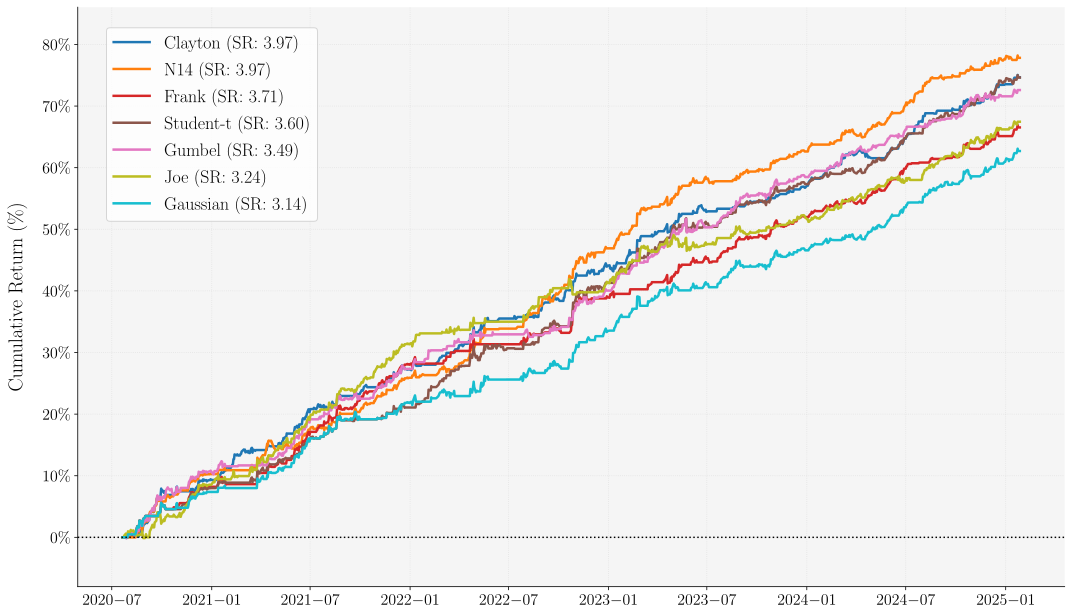
\includegraphics[width=0.9\linewidth,height=\textheight,keepaspectratio]{simple_Presentation_files/mediabag/images/converted/equity_curves_comparison.pdf}
\end{center}

\subsection{Factor analysis of Strategy
Returns}\label{factor-analysis-of-strategy-returns}

For each copula model, we run the regression \[
\mathcal{R}_{t}^{c} = \alpha + \boldsymbol{\beta}' \mathbf{f}_t + \epsilon_t
\]

\begin{itemize}
\tightlist
\item
  \(\mathcal{R}_{t}^{c}\equiv\) excess returns of our pairs trading
  strategy for copula family \(c\)
\item
  \(\mathbf f_t \equiv\) \textbf{Fama-French Factors}:

  \begin{itemize}
  \tightlist
  \item
    \(\texttt{MKT_RF}\): Market factor
  \item
    \(\texttt{SMB}\): Size factor
  \item
    \(\texttt{HML}\): Value factor
  \item
    \(\texttt{RMW}\): Profitability factor
  \item
    \(\texttt{CMA}\): Investment factor
  \item
    \(\texttt{MOM}\): Momentum factor
  \item
    \(\texttt{ST_REV}\): Short-term reversal factor
  \item
    \(\texttt{LT_REV}\): Long-term reversal factor
  \end{itemize}
\end{itemize}

\subsection{Factor analysis of Strategy
Returns}\label{factor-analysis-of-strategy-returns-1}

\[
\mathcal{R}_{t}^{c} = \alpha + \boldsymbol{\beta}' \mathbf{f}_t + \epsilon_t
\]

\begin{itemize}
\tightlist
\item
  Since we consider combinations of 8 factors, we run \(2^8=256\)
  different regressions for each copula.
\item
  This delivers a positive significant \(\alpha\) of \(0.0004\) --
  \(0.0006\) for all regressions specifications across all copula
  models, which is equivalent to an annualized \(\alpha\) of \(10.08\%\)
  -- \(15.12\%\).
\item
  The significance of risk-factors varies through copula models.
\end{itemize}

\subsection{Factor analysis of Strategy
Returns}\label{factor-analysis-of-strategy-returns-2}

\begin{itemize}
\tightlist
\item
  Gumbel copula strategy returns

  \begin{itemize}
  \tightlist
  \item
    limited factor exposure to SMB, HML and ST\_REV
  \item
    the overall factor model reliability is questionable though
  \end{itemize}
\end{itemize}

\begin{itemize}
\tightlist
\item
  Frank copula strategy returns

  \begin{itemize}
  \tightlist
  \item
    significant exposure primarily to the Short-term Reversal (ST\_REV)
  \end{itemize}
\end{itemize}

\begin{itemize}
\tightlist
\item
  Clayton copula strategy returns

  \begin{itemize}
  \tightlist
  \item
    significantly exposed to market risk, with MKT\_RF being the sole
    statistically significant factor across all model specifications.
  \end{itemize}
\end{itemize}

\begin{itemize}
\tightlist
\item
  Joe copula strategy returns

  \begin{itemize}
  \tightlist
  \item
    mild sensitivity to market risk
  \end{itemize}
\end{itemize}

\subsection{Factor analysis of Strategy
Returns}\label{factor-analysis-of-strategy-returns-3}

\begin{itemize}
\tightlist
\item
  N14 copula strategy returns

  \begin{itemize}
  \tightlist
  \item
    significant exposure to the market factor.
  \item
    The model's explanatory power improves notably when incorporating
    the Short-term Reversal factor.
  \end{itemize}
\end{itemize}

\begin{itemize}
\tightlist
\item
  Gaussian copula strategy returns

  \begin{itemize}
  \tightlist
  \item
    significant exposure to market risk and ST\_REV (significant at the
    1\% level).
  \end{itemize}
\end{itemize}

\begin{itemize}
\tightlist
\item
  Student-t copula strategy returns

  \begin{itemize}
  \tightlist
  \item
    mild sensitivity to the Profitability factor (RMW), suggesting the
    potential relevance of a single-factor model focused solely on RMW.
  \end{itemize}
\end{itemize}

\section{Conclusion}\label{conclusion}

\subsection{Conclusions}\label{conclusions}

\begin{itemize}
\tightlist
\item
  We proposed a novel approach to detect pricing anomalies in the
  context of pairs trading
\item
  Our framework combines sparse synthetic control methods with
  copula-based dependence modeling
\item
  Our empirical application demonstrate the effectiveness of our trading
  strategy
\item
  The strategy is robust across different copula specifications
\end{itemize}

\subsection{TO-DOs}\label{to-dos}

\begin{itemize}
\tightlist
\item
  Robustness checks:

  \begin{itemize}
  \tightlist
  \item
    Run this procedure by looping the target asset through all the S\&P
    500 constituents
  \item
    Explore different train-test split percentages
  \item
    Run strategy on multiple paths (\emph{Combinatorial Purged
    Cross-Validation})
  \end{itemize}
\end{itemize}

\begin{itemize}
\tightlist
\item
  Investigate the spread between the target and synthetic assets (Barra
  model)
\end{itemize}

\begin{itemize}
\tightlist
\item
  Is Fama-French factor analysis on the strategy returns valid in my
  context?
\end{itemize}

\begin{itemize}
\tightlist
\item
  Incorporate transaction costs
\end{itemize}

\begin{itemize}
\tightlist
\item
  Explore time-varying copulas(?)
\end{itemize}




\end{document}
